\begin{figure}[ht!]
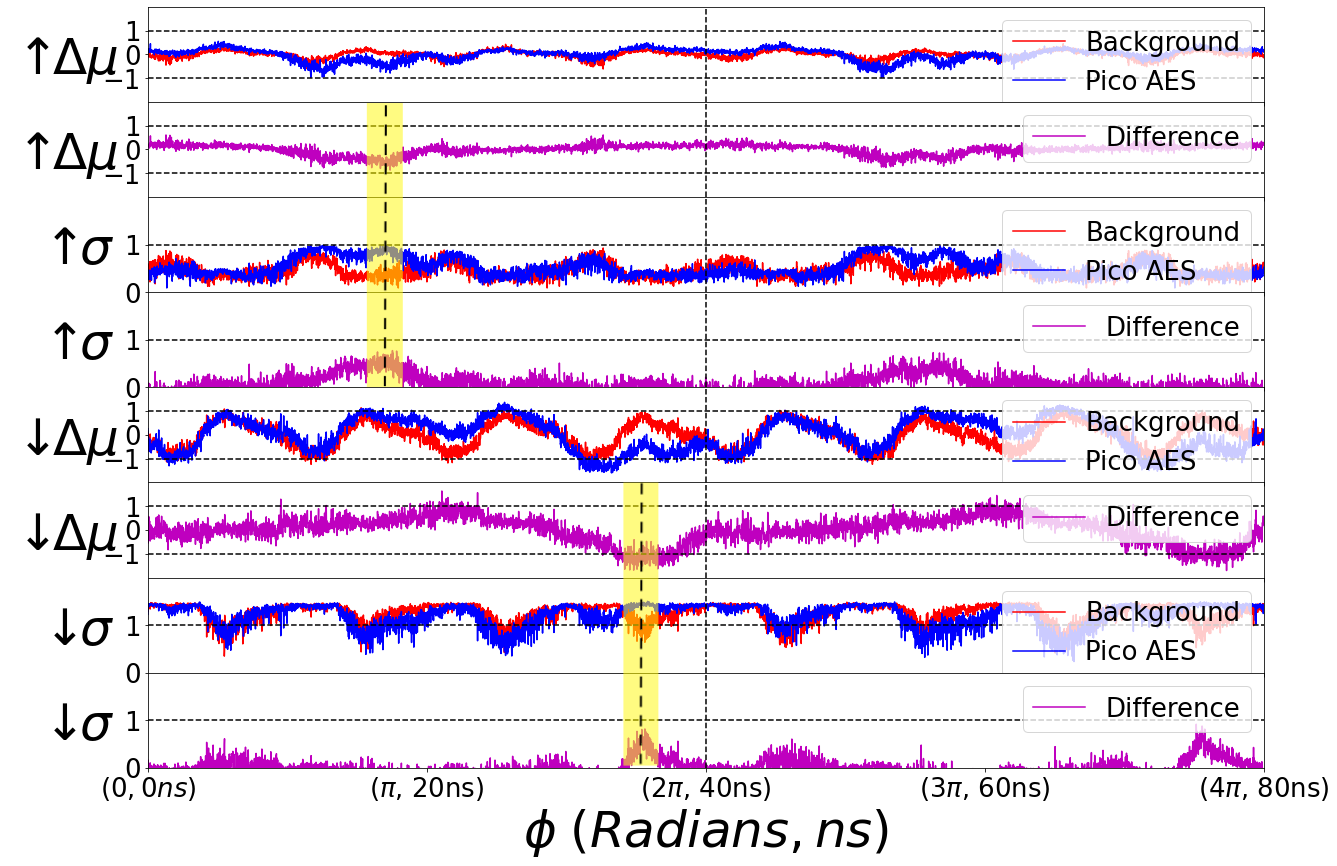
\includegraphics[width=\linewidth]{img/pico_aes_DIFF_pynq_std_ham_pn_4pi.png}
\vspace{-20px}
\caption{Measuring sensor output as $\phi$ is swept from 0 to 4$\pi$ on PYNQ-Z2 PicoRV AES design. Background subtraction is necessary to isolate a target from other information sources on the system and reveal the value of $\phi$ where the side channel between the target and the sensor is maximized.}
\label{fig:phi-pynq-pico}
\vspace{-15px}
\end{figure} 
